\documentclass{article}
\usepackage[utf8]{inputenc}
\usepackage{graphicx}

\begin{document}

\section{System Monitor}

\subsection{Objective and Functionality}
The System Monitor is a pivotal component in a biometric data-based framework for user access and verification. It serves two main functions: position detection using user location data and user identification. The System Monitor's functionalities include:
\begin{itemize}
    \item Subscribing to and processing location data from two ESP-01 modules with ultrasonic sensors via MQTT.
    \item Displaying user location and verification data on an LCD screen.
    \item Visually representing user proximity using an LED bar.
\end{itemize}

\subsection{Project Definition and Milestones}
The development of the System Monitor involved the following milestones:
\begin{enumerate}
    \item Establishing MQTT communication to receive data from ultrasonic sensors.
    \item Integrating and configuring the LED bar and LCD with the ESP32.
    \item Developing and testing the software for proximity detection and data display.
    \item Efficient multitasking and task synchronization within FreeRTOS.
\end{enumerate}

\subsection{Milestones Execution Order, Priority, and Dependencies}
\begin{enumerate}
    \item \textbf{Milestone 1: Establishing MQTT Communication}
       - \textit{Priority:} High. Fundamental for data transmission.
       - \textit{Dependencies:} Basic WiFi setup.
       - \textit{Execution Order:} First, as it is crucial for data reception.

    \item \textbf{Milestone 2: LED Bar and LCD Integration}
       - \textit{Priority:} Medium. Important for user interface.
       - \textit{Dependencies:} Successful MQTT setup.
       - \textit{Execution Order:} Second, building upon established communication.

    \item \textbf{Milestone 3: Software Development}
       - \textit{Priority:} High. Essential for functionality.
       - \textit{Dependencies:} Functional hardware setup.
       - \textit{Execution Order:} Third, focusing on processing and display.

    \item \textbf{Milestone 4: Multitasking and Task Synchronization}
       - \textit{Priority:} High. Critical for system reliability.
       - \textit{Dependencies:} Completion of initial software development.
       - \textit{Execution Order:} Fourth, finalizing the system integration.
\end{enumerate}ƒ

\subsection{Hardware Development}
The hardware setup for the System Monitor comprises:
\begin{itemize}
    \item An ESP32 microcontroller connected to a breadboard.
    \item An LED bar and an LCD screen interfaced with the ESP32 for display.
    \item Two ESP-01 modules, each with an ultrasonic sensor, for distance measurement.
\end{itemize}

\subsection{Software Implementation}
The software, written in C++, leverages FreeRTOS for effective multitasking. Key functions include:
\begin{itemize}
    \item \texttt{WiFiTask} for managing WiFi connectivity.
    \item \texttt{MQTTTask} for handling MQTT communication.
    \item \texttt{LCDDisplayTask} and \texttt{checkForPresenceAndDirection} for controlling the display based on sensor data.
    \item Semaphore (\texttt{xSemaphoreLCD}) to ensure safe LCD access.
\end{itemize}

\subsection{Interaction with Other Components}
The System Monitor interacts with the ESP-01 modules to determine the user's location based on distance data, which is then displayed on the LED bar and LCD screen.

\subsection{Testing}
Testing ensured accurate sensor data transmission via MQTT and responsive displays on the LED bar and LCD. An iterative approach was applied to refine the system's performance.

\subsection{Dedication Time}
Approximately 20 hours were dedicated to developing the System Monitor, focusing on both hardware assembly and software programming.

\subsection{User Story}
As a user approaches, the System Monitor detects their presence, lighting up the LED bar and displaying their approximate location (left, right, or center) on the LCD screen, providing real-time feedback.

\subsection{Challenges and Solutions}
\begin{itemize}
    \item \textbf{Hardware Challenges:} Complex wiring and space constraints on the breadboard, along with troubleshooting LED issues.
    \item \textbf{Software Challenges:} Establishing reliable communication and processing sensor data accurately. Achieved through careful coding and testing.
\end{itemize}

\subsection{Hardware and Software Integration}
\begin{figure}[ht]
    \centering
    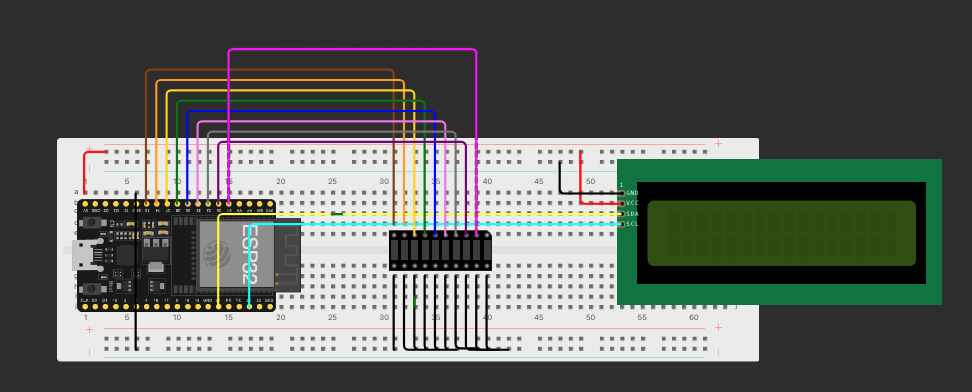
\includegraphics[width=0.8\textwidth]{../images/activity_monitor_scheme.png}
    \caption{ESP32 with LED bar and LCD display connected on a breadboard.}
    \label{fig:esp32_system_monitor}
\end{figure}

\subsection{Microcontroller Interaction Protocol}
The System Monitor project involves coordinated communication between multiple microcontrollers, primarily the ESP32 and two ESP-01 modules. The communication is structured as follows:

\subsubsection{Communication Protocol}
The project utilizes the MQTT (Message Queuing Telemetry Transport) protocol, a lightweight and efficient messaging protocol ideal for IoT applications. This protocol is chosen for its low bandwidth usage and its ability to provide reliable communication over WiFi.

\subsubsection{WiFi Configuration}
Each microcontroller in the system is configured to connect to a WiFi network, enabling them to send and receive data over the network. The network credentials (SSID and password) are programmed into the microcontrollers.

\subsubsection{Data Flow and Configuration}
The ESP-01 modules, each equipped with an ultrasonic sensor, collect distance data and publish this information to specific MQTT topics. The ESP32, acting as the central unit, subscribes to these topics to receive the data.

\subsection{MQTT Tree Structure}
The MQTT protocol in the System Monitor project uses a structured approach to manage the data flow. Below is the outline of the MQTT topics and their functions:

\subsubsection{MQTT Topics}
\begin{itemize}
    \item \textbf{sensor1/distance:} This topic is used by the first ESP-01 module. It publishes the distance data measured by its connected ultrasonic sensor. The ESP32 subscribes to this topic to receive updates on the user's distance from this sensor.
    \item \textbf{sensor2/distance:} Similar to the first, this topic is for the second ESP-01 module. It provides distance data from its sensor, allowing the ESP32 to determine the user's location relative to this second sensor.
\end{itemize}

\subsubsection{Data Organization and Utilization}
The data sent to these topics include numerical values representing the measured distances. The ESP32, upon receiving this data, processes it to determine the user's proximity and location. Based on these calculations, the ESP32 then controls the LED bar and the LCD display to provide real-time feedback about the user's position.

\end{document}
